\chapter{静态无向模型}
\label{chap:pgm-energy-models}

相邻检测位置可能同时过热，也可能受到同一测量干扰，整排状态因而需要联合考虑。给定各位置的相对偏好以及相邻状态的相容权重，怎样计算整排配置的概率？若温度读数已知、只需预测异常标签，是否还要同时建立这些读数的生成分布？

两项任务都可以组合局部势，区别在于哪些变量参与归一化。联合无向模型比较全部建模变量的配置，条件无向模型则固定输入、只比较输出。局部无向分解规定了变量在给定分隔节点后的独立关系（参见第~\ref{chap:pgm-undirected}章）；本章据此构造具体模型，说明结构怎样影响推断，以及潜变量、高阶势和神经参数化各带来哪些表达能力与计算要求。联合与条件是本章的主要划分；变量是否可见、势是否成对以及参数化方式可以组合。

\section{无向模型的共同形式}
\label{sec:pgm-energy-models-common}

先为整排状态规定无向图$\mathcal{G}=(V,E)$，令$d=|V|$、$\bm{X}=(X_1,\ldots,X_d)^\top$。局部配置越符合建模偏好，其\term{势函数}（potential function）值越大；这个值表示相对相容程度，无须自身求和为$1$。记因子作用域集合为$\mathcal{C}$，每个$C\in\mathcal{C}$取图中的一个团，允许使用非极大团。将严格正势$\psi_{\bm{\theta},C}$写成局部能量$E_{\bm{\theta},C}=-\log\psi_{\bm{\theta},C}$，乘积权重便转为能量之和：
\begin{equation}
  \begin{aligned}
    E_{\bm{\theta}}(\bm{x})
      &=\sum_{C\in\mathcal{C}}E_{\bm{\theta},C}(\bm{x}_C),\\
    p_{\bm{\theta}}(\bm{x})
      &=\frac{\prod_{C\in\mathcal{C}}
               \psi_{\bm{\theta},C}(\bm{x}_C)}
              {Z_{\bm{\theta}}}
        =\frac{\exp[-E_{\bm{\theta}}(\bm{x})]}{Z_{\bm{\theta}}},\\
    Z_{\bm{\theta}}
      &=\int \exp[-E_{\bm{\theta}}(\bm{u})]\,\mathrm{d}\mu(\bm{u}).
  \end{aligned}
  \label{eq:pgm-energy-models-joint}
\end{equation}
参数向量$\bm{\theta}$包含各局部势的参数。离散状态采用计数测度$\mu$，连续状态采用指定基准测度，通常是Lebesgue测度。\term{能量函数}（energy function）的值越低，配置的未归一化权重越大；\term{配分函数}（partition function）$Z_{\bm{\theta}}$累加或积分全部权重，使其成为概率，故须满足$0<Z_{\bm{\theta}}<\infty$。这里使用无量纲的对数权重，物理模型的逆温度已计入参数。

也可以用负能量$f_{\bm{\theta}}=-E_{\bm{\theta}}$给配置评分，对数概率还需扣除$\log Z_{\bm{\theta}}$。增加与$\bm{x}$无关的能量常数，会等比例缩放全部权重及配分函数，概率保持原值；正数缩放能量则通常改变概率的集中程度。若只比较固定模型中的两种配置，配分函数可从比值中消去：
\[
  \frac{p_{\bm{\theta}}(\bm{x})}{p_{\bm{\theta}}(\bm{x}')}
  =\exp\{E_{\bm{\theta}}(\bm{x}')-E_{\bm{\theta}}(\bm{x})\}.
\]
因此，能量差能够排序配置，绝对概率仍依赖全部权重的总量。改变一个局部势的状态偏好时，配分函数通常也会改变；即使其他局部势未变，其对应配置的概率也可能随归一化而改变。

若测量输入$\bm{x}$已经固定、待预测量为$\bm{Y}$，需要比较的候选只有输出配置。相同能量构造此时只在输出空间归一化：
\begin{equation}
  \begin{aligned}
    p_{\bm{\theta}}(\bm{y}\mid\bm{x})
      &=\frac{\exp[-E_{\bm{\theta}}(\bm{y},\bm{x})]}
              {Z_{\bm{\theta}}(\bm{x})},\\
    Z_{\bm{\theta}}(\bm{x})
      &=\int\exp[-E_{\bm{\theta}}(\bm{v},\bm{x})]
                  \,\mathrm{d}\mu_Y(\bm{v}).
  \end{aligned}
  \label{eq:pgm-energy-models-conditional}
\end{equation}
每个使用的输入都须给出$0<Z_{\bm{\theta}}(\bm{x})<\infty$。该式只定义输出的条件概率，没有为输入规定$p(\bm{x})$，也不限制输入之间的依赖。附加只依赖输入的能量$c(\bm{x})$时，它在分子、分母中消去。图~\ref{fig:pgm-energy-models-normalization}据此区分输入的两种职责：它可以改变各势的数值，却不参与输出的求和。

\begin{figure}[htbp]
  \centering
  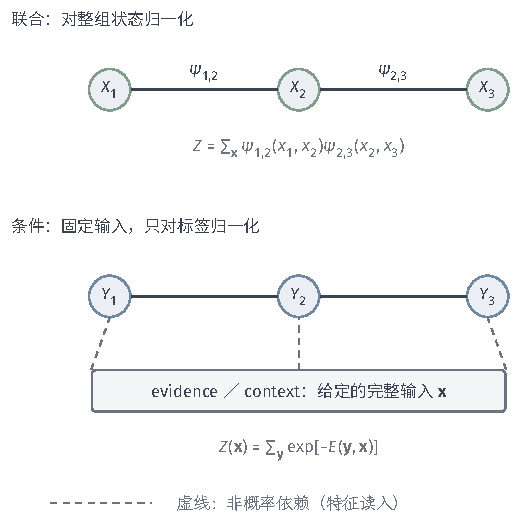
\includegraphics[width=86.907mm]{figures/06-probabilistic-graphical-models/04-models/tikz/pgm-energy-models-normalization/figure.pdf}
  \caption{三节点相互作用的两种归一化。上方联合模型对全部状态求和；下方把$\bm{x}$列为给定证据或条件输入，只对标签$\bm{y}$求和。灰底框中的输入通过虚线影响标签势，虚线表示特征依赖，不表示有向生成关系。}
  \label{fig:pgm-energy-models-normalization}
\end{figure}

有限离散状态配合有限能量，必然产生正且有限的配分函数。连续能量则需检查尾部：即使$E(x)=-x^2$处处有定义，$\int_{\mathbb{R}}e^{x^2}\,\mathrm{d}x$仍发散。允许势为零时，可以用$+\infty$能量排除配置，但归一化还须有正总权重；离散支持至少保留一个正权配置，连续支持则需有正测度。因子分解仍能给出相应Markov性质，而从Markov性质反推分解的正性定理不能直接用于零势（参见第~\ref{chap:pgm-undirected}章）。

\section{联合能量模型}
\label{sec:pgm-energy-models-joint-models}

补全状态、计算多变量事件或生成整组配置，都需要联合分布。以下先取成对作用，再分别引入隐藏状态、改变能量函数或扩大因子作用域。它们共同使用式~\eqref{eq:pgm-energy-models-joint}，推断时能利用的分解与代数形式却各不相同。

\subsection{观测变量成对模型}
\label{sec:pgm-energy-models-pairwise}

对只有两种状态的检测位置，取$x_i\in\{-1,+1\}$。\term{Ising模型}（Ising model）分别用单点参数表示状态偏好，用边参数表示相邻状态同号或异号的偏好：
\begin{equation}
  E_{\bm{\theta}}(\bm{x})
    =-\sum_{i\in V}b_ix_i
     -\sum_{\{i,j\}\in E}J_{i,j}x_ix_j.
  \label{eq:pgm-energy-models-ising}
\end{equation}
\term{外场}（external field）$b_i$取正值时偏好$+1$。\term{耦合参数}（coupling parameter）$J_{i,j}$取正值时奖励同号，取负值时奖励异号；每条无向边只计一次，约定$J_{i,j}=J_{j,i}$。这些参数描述统计相容性，不能仅凭它们推断干预一个位置对另一位置的效应。

要计算一个位置的条件概率，固定其余状态，仅保留含$x_i$的得分$x_i(b_i+\sum_{j\in N(i)}J_{i,j}x_j)$，其中$N(i)$为邻居集合。$+1$与$-1$的权重比为$\exp[2(b_i+\sum_jJ_{i,j}x_j)]$，归一化两项后得到
\begin{equation}
  \begin{aligned}
    p_{\bm{\theta}}(X_i=+1\mid\bm{x}_{V\setminus\{i\}})
      &=\sigma\!\left(2b_i+
           2\sum_{j\in N(i)}J_{i,j}x_j\right),\\
    \sigma(u)&=\frac{1}{1+e^{-u}}.
  \end{aligned}
  \label{eq:pgm-energy-models-ising-conditional}
\end{equation}
这个满条件分布只读取邻居状态。移去这些条件以后，无直接边的两个节点仍可能经其他节点相关。

用三个相邻位置构造数值例子：图取$1-2-3$，不设单点偏好，同号边势为$3$、异号边势为$1$。这些是人为指定的权重，尚未归一化为概率。为计算联合权重，先统计相邻同号对：
\[
  N_{=}(\bm{x})
   =\mathbf{1}\{x_1=x_2\}+\mathbf{1}\{x_2=x_3\}.
\]
令$E_0(\bm{x})=-(\log3)N_{=}(\bm{x})$，配置权重就是$3^{N_{=}(\bm{x})}$。首节点可取两个值，每个后继节点的两项权重和为$3+1=4$，故$Z_0=2\times4\times4=32$。由$\mathbf{1}\{x_i=x_j\}=(1+x_ix_j)/2$，这也对应$J_{1,2}=J_{2,3}=(\log3)/2$的Ising分布。两种能量约定相差常数：$E_0$比式~\eqref{eq:pgm-energy-models-ising}的零外场能量少$\log3$，后者的配分函数为$32/3$。概率相同，配分函数数值则随能量常数而变。

在该对称链中，给定一个位置，后继位置同号和异号的条件概率分别为$3/4$、$1/4$。两端同号对应两次保持或两次翻转，因而
\[
  p(X_3=X_1\mid X_1)
    =(3/4)^2+(1/4)^2=\frac58.
\]
各节点的边缘都为均匀二值分布，所以$\mathbb{E}[X_1X_3]=2(5/8)-1=1/4$。两端虽无边仍相关，给定$X_2$才独立。将同样参数用于更长的零外场链，每跨一条边，条件均值乘以$1/2$，相隔$r$条边的相关为$(1/2)^r$。这说明相互作用能够沿路径传递，其强度还由参数决定。

类别数增加到$K>2$后，标签编号的乘积无法直接表示相容性。\term{Potts模型}（Potts model）改为比较类别是否相等，对$x_i\in\{1,\ldots,K\}$定义
\begin{equation}
  E_{\bm{\theta}}(\bm{x})
   =-\sum_i b_i(x_i)
    -\sum_{\{i,j\}\in E}J_{i,j}\mathbf{1}\{x_i=x_j\}.
  \label{eq:pgm-energy-models-potts}
\end{equation}
$b_i(k)$规定位置$i$对类别$k$的偏好。计算节点条件分布时，固定邻居，为每个类别$k$形成权重
\[
  w_i(k)=\exp\left\{
    b_i(k)+\sum_{j\in N(i)}J_{i,j}\mathbf{1}\{k=x_j\}
  \right\},
\]
将权重除以$\sum_{\ell=1}^K w_i(\ell)$即得满条件概率。每条边只用一个参数区分类别相同与不同，限制了它能表达的相容关系；特定异类组合有不同偏好时，需改用$K\times K$边势表。二类Potts可以重新编码为Ising，其中耦合系数需按前述$1/2$因子换算。

完整观测提供单点状态以及边上的乘积或同类指示。固定图、存在有限内点最大似然解时，模型期望与对应经验统计量匹配；例如$J_{i,j}$的似然梯度使用经验$x_ix_j$减去$\mathbb{E}[X_iX_j]$（通用推导及替代准则参见第~\ref{chap:pgm-parameter-learning}章）。Ising的解析满条件还能直接用于Gibbs更新和伪似然拟合。强耦合时，单点变化难以转到另一种整体配置，采样仍可能很慢。

一般稠密边势在树上求配分函数与边缘需$O(dK^2)$运算，特殊边势可能进一步简化。一般图则受消元后的诱导宽度限制，原始因子成对不保证全局计算只有二次成本。二值吸引型模型可以通过图割求最优配置，但这一最大化未计算配分函数（参见第~\ref{chap:pgm-variational}章）。参数也会限制模型适用性：过强的同号偏好可能掩盖局部异常；三角形的每条边都偏好异号时，任一二值配置至少违背一项偏好。

温度等连续状态可以用二次能量描述。\term{高斯Markov随机场}（Gaussian Markov random field, GMRF）通过精度矩阵表示条件依赖；对$\bm{x}\in\mathbb{R}^d$取
\begin{equation}
  \begin{aligned}
    E_{\bm{\theta}}(\bm{x})
      &=\frac12(\bm{x}-\bm{\mu})^\top
                    \bm{Q}(\bm{x}-\bm{\mu}),\\
    Z_{\bm{\theta}}
      &=(2\pi)^{d/2}|\bm{Q}|^{-1/2},
      \qquad \bm{Q}=\bm{Q}^\top\succ0.
  \end{aligned}
  \label{eq:pgm-energy-models-gaussian}
\end{equation}
均值为$\bm{\mu}$，协方差的逆$\bm{Q}$称为\term{精度矩阵}（precision matrix）。正定性使二次能量在所有方向增长，并使高斯积分有限。为补全一个未知位置，给定其余位置后的分布为
\[
  \begin{aligned}
    \widetilde{\mu}_i(\bm{x})
      &=\mu_i-\frac{1}{Q_{i,i}}
           \sum_{j\ne i}Q_{i,j}(x_j-\mu_j),\\
    X_i\mid\bm{x}_{V\setminus\{i\}}
      &\sim\mathcal{N}\!\left(
          \widetilde{\mu}_i(\bm{x}),Q_{i,i}^{-1}\right).
  \end{aligned}
\]
$\widetilde{\mu}_i$是给定其余节点后的条件均值。在非退化高斯模型中，$Q_{i,j}=0$恰好对应$X_i\perp X_j\mid\bm{X}_{V\setminus\{i,j\}}$；协方差为零判别的则是边缘独立，两者不可互换（证明参见第~\ref{chap:pgm-undirected}章）。

仍取三个检测位置，用中心化并缩放后的温度构造零均值模型，令
\[
  \bm{Q}=
  \begin{pmatrix}
    2&-1&0\\ -1&2&-1\\ 0&-1&2
  \end{pmatrix},
  \qquad
  \bm{Q}^{-1}=\frac14
  \begin{pmatrix}
    3&2&1\\ 2&4&2\\ 1&2&3
  \end{pmatrix}.
\]
$\bm{Q}$的顺序主子式为$2,3,4$，所以它正定。两端精度为零，协方差却为$1/4$，展示了中点传递的边缘相关。给定$x_1=2,x_3=0$，中点分布为$\mathcal{N}(1,1/2)$；以条件均值补全得到$1$，条件方差则量化补全后仍有的不确定性。

高斯推断主要使用线性求解和矩阵分解。稠密Cholesky分解耗时$O(d^3)$，随后可计算条件均值、所需协方差及对数行列式；链状精度具有固定带宽时，分解可随$d$线性增长。一般稀疏矩阵可能产生消元填充，原始零元素数量因此不足以判定时间成本。学习时，若均值已知为零，取样本二阶矩$\bm{S}=n^{-1}\sum_{r=1}^n\bm{x}_r\bm{x}_r^\top$，要最大化的精度相关对数似然为
\[
  \frac n2\{\log|\bm{Q}|-\operatorname{tr}(\bm{S}\bm{Q})\},
  \qquad \bm{Q}\succ0,
\]
缺边对应$Q_{i,j}=0$，这些约束与正定性共同限定候选精度。无图约束且$\bm{S}\succ0$时，最优解是$\bm{S}^{-1}$；有零约束时通常需要约束优化。仅半正定的精度不能在整个$\mathbb{R}^d$上归一化为式~\eqref{eq:pgm-energy-models-gaussian}，单个高斯也无法表达多峰。解析计算的便利伴随这些表示条件，延长优化迭代不能消除它们\scite{pgm-undirected-rue2005}

\subsection{潜变量能量模型}
\label{sec:pgm-energy-models-latent}

共同异常也可能来自未测状态。可以让一个潜变量连接多个可见位置，先建立联合分布，再将它边缘化。\term{玻尔兹曼机}（Boltzmann machine, BM）采用二值变量的成对能量实现这一构造。以下改用$0/1$编码：可见量为$\bm{x}\in\{0,1\}^{d_{\mathrm{v}}}$，隐藏量为$\bm{z}\in\{0,1\}^m$，共有$d_{\mathrm{v}}+m$个节点：
\begin{equation}
  \begin{aligned}
    E_{\bm{\theta}}(\bm{x},\bm{z})
      &=-\bm{b}^\top\bm{x}-\bm{c}^\top\bm{z}
        -\bm{x}^\top\bm{W}\bm{z}\\
      &\quad-\frac12\bm{x}^\top\bm{U}\bm{x}
             -\frac12\bm{z}^\top\bm{R}\bm{z},\\
    p_{\bm{\theta}}(\bm{x},\bm{z})
      &=\frac{e^{-E_{\bm{\theta}}(\bm{x},\bm{z})}}
               {Z_{\bm{\theta}}},\\
    p_{\bm{\theta}}(\bm{x})
      &=\sum_{\bm{z}}p_{\bm{\theta}}(\bm{x},\bm{z}).
  \end{aligned}
  \label{eq:pgm-energy-models-bm}
\end{equation}
$\bm{W}\in\mathbb{R}^{d_{\mathrm{v}}\times m}$连接可见与隐藏节点，$\bm{U}$、$\bm{R}$分别连接各组内部，二者对称且对角为零。组内项乘$1/2$以避免重复计边。一般BM即使固定全部可见量，隐藏节点仍有相互作用；训练所需的数据后验期望和无条件模型期望都可能依赖近似推断。

若要直接计算隐藏后验，可以删除两组各自内部的边，令$\bm{U}=\bm{0}$、$\bm{R}=\bm{0}$。这就是\term{受限玻尔兹曼机}（restricted Boltzmann machine, RBM）的二部限制：固定一组以后，另一组的节点没有剩余相互作用。记$u_j(\bm{x})=c_j+\sum_iW_{i,j}x_i$，隐藏条件分布分解为
\[
  p_{\bm{\theta}}(\bm{z}\mid\bm{x})
   =\prod_{j=1}^m\frac{\exp[z_ju_j(\bm{x})]}
                         {1+\exp[u_j(\bm{x})]}.
\]
每个分母都由$z_j=0,1$的两个权重相加得到，条件分布因而按节点独立。交换两组可得相应的可见条件分布：
\begin{equation}
  \begin{aligned}
    p_{\bm{\theta}}(Z_j=1\mid\bm{x})
      &=\sigma\!\left(c_j+\sum_iW_{i,j}x_i\right),\\
    p_{\bm{\theta}}(X_i=1\mid\bm{z})
      &=\sigma\!\left(b_i+\sum_jW_{i,j}z_j\right).
  \end{aligned}
  \label{eq:pgm-energy-models-rbm-conditionals}
\end{equation}
这些sigmoid表达没有Ising满条件的系数$2$，因为变量已经由$\{-1,+1\}$改为$0/1$编码。

二部限制还简化了隐藏变量的求和。对固定可见配置，\term{自由能}（free energy）取全部隐藏配置权重和的负对数，得到可见分布的有效能量；它汇总隐藏状态，而非只取最优隐藏状态：
\begin{equation}
  \begin{aligned}
    F_{\bm{\theta}}(\bm{x})
      &:=-\log\sum_{\bm{z}}
                 e^{-E_{\bm{\theta}}(\bm{x},\bm{z})}\\
      &=-\bm{b}^\top\bm{x}
        -\sum_{j=1}^m\log(1+e^{u_j(\bm{x})}),\\
    p_{\bm{\theta}}(\bm{x})
      &=\frac{e^{-F_{\bm{\theta}}(\bm{x})}}{Z_{\bm{\theta}}}.
  \end{aligned}
  \label{eq:pgm-energy-models-free-energy}
\end{equation}
隐藏求和可拆成$\sum_{\bm{z}}\prod_j e^{z_ju_j}=\prod_j(1+e^{u_j})$，这给出了自由能公式。隐藏节点连接多个可见节点时，消元后的一项$\log(1+e^{u_j})$通常同时依赖它们。因此，联合模型中的成对作用可以成为可见边缘中的高阶势（图~\ref{fig:pgm-energy-models-rbm}）。

\begin{figure}[htbp]
  \centering
  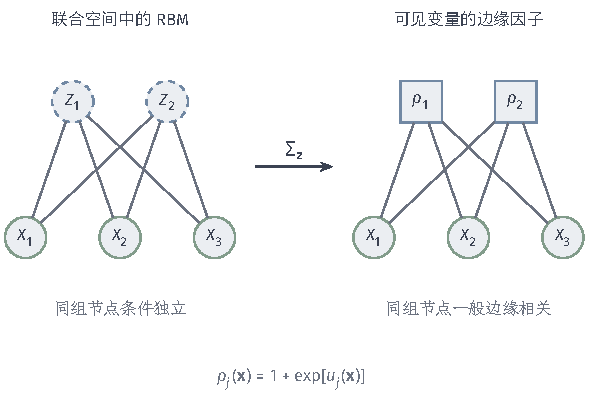
\includegraphics[width=99.653mm]{figures/06-probabilistic-graphical-models/04-models/tikz/pgm-energy-models-rbm/figure.pdf}
  \caption{RBM的条件分解与隐藏消元。左侧仅有跨组边，固定一组时另一组条件独立；右侧把两个隐藏节点消去，两个因子$1+\exp[u_j(\bm{x})]$各涉及三个可见变量。一元可见偏置势在两侧均省略。可见边缘仍可能相关。}
  \label{fig:pgm-energy-models-rbm}
\end{figure}

取两个可见节点和一个隐藏节点，偏置均为零，$W_{1,1}=W_{2,1}=\log2$。可见权重为$e^{-F(\bm{x})}=1+2^{x_1+x_2}$，配置$(0,0),(0,1),(1,0),(1,1)$的权重依次为$2,3,3,5$，总和为$13$。给定$(x_1,x_2)=(1,1)$，隐藏状态为$1$的概率是$4/5$。给定$z=0$时，两可见节点独立、取$1$概率各为$1/2$；给定$z=1$时，该概率各为$2/3$。消去隐藏状态后，$p(X_1=X_2=1)=5/13$与$p(X_1=1)p(X_2=1)=(8/13)^2$相差$1/169$，独立性没有保留。

单个可见配置的自由能求值为$O(d_{\mathrm{v}}m)$，其权重总和$Z_{\bm{\theta}}=\sum_{\bm{x}}e^{-F_{\bm{\theta}}(\bm{x})}$通常仍需指数计算。枚举较小的一组、解析消去另一组虽可减少运算，仍含$2^{\min(d_{\mathrm{v}},m)}$规模。RBM使完整可见配置下的隐藏后验可算，没有普遍消除联合归一化成本。部分可见量未测时，$p(\bm{z}\mid\bm{x}_{\mathrm{obs}})$也未必保有上述独立Bernoulli分解。

这两个块条件可以构成\term{交替Gibbs采样}（alternating Gibbs sampling）：固定一组，独立随机抽取另一组，再交换两组。算法~\ref{alg:pgm-energy-models-rbm-gibbs}传递的是抽到的二值状态；若直接传递概率，所得确定性迭代已不再使用这个Gibbs核。

\begin{algorithm}[RBM的一段交替Gibbs链]
  \label{alg:pgm-energy-models-rbm-gibbs}
  \begin{algorithmic}[1]
    \Require 固定的有限参数$\bm{\theta}$，初始状态$\bm{x}^{(0)}$，步数$k\geq1$
    \Ensure 链状态$\bm{x}^{(1)},\ldots,\bm{x}^{(k)}$
    \For{$t=0,\ldots,k-1$}
      \State 按式~\eqref{eq:pgm-energy-models-rbm-conditionals}独立抽取各$Z_j^{(t+1)}$
      \State 固定$\bm{z}^{(t+1)}$，独立抽取各$X_i^{(t+1)}$
    \EndFor
  \end{algorithmic}
\end{algorithm}

固定有限参数下，每个块条件概率都在$0$与$1$之间，可见状态链因而能到达任意配置，并有自转移。交替Gibbs核保持$p_{\bm{\theta}}(\bm{x})$不变，有限不可约、非周期链的分布遂长期收敛到它；这并未给出小$k$充分混合的保证（参见第~\ref{chap:pgm-sampling}章）。完整一次更新为$O(d_{\mathrm{v}}m)$，强权重形成的近确定条件可能使链长期停留在同一模式。

训练一个权重时，需要提高数据配置的概率，同时扣除模型自身的联合统计。对单条数据$\bm{x}$，潜变量似然梯度在RBM中写为（通用推导参见第~\ref{chap:pgm-parameter-learning}章）
\begin{equation}
  \frac{\partial\log p_{\bm{\theta}}(\bm{x})}
       {\partial W_{i,j}}
    =x_i\,p_{\bm{\theta}}(Z_j=1\mid\bm{x})
      -\mathbb{E}_{p_{\bm{\theta}}}[X_iZ_j].
  \label{eq:pgm-energy-models-rbm-gradient}
\end{equation}
数据项由隐藏条件概率精确取得，模型项则通常需要采样。多条记录对数据项求平均，偏置的梯度对应一阶统计量。RBM简化的是给定数据的后验计算，模型期望仍然存在。重构误差与似然也有不同含义：慢混合的短链容易留在起始数据附近，却可能没有正确分配不同模式的概率质量\scite{pgm-energy-models-hinton2010}

图~\ref{fig:rbm-alternating-sampling-and-gradient}按这一顺序区分概率、抽样状态与训练统计：先固定参数运行交替链、估计模型统计，再用数据统计减模型统计更新参数。

\begin{figure*}[htbp]
  \centering
  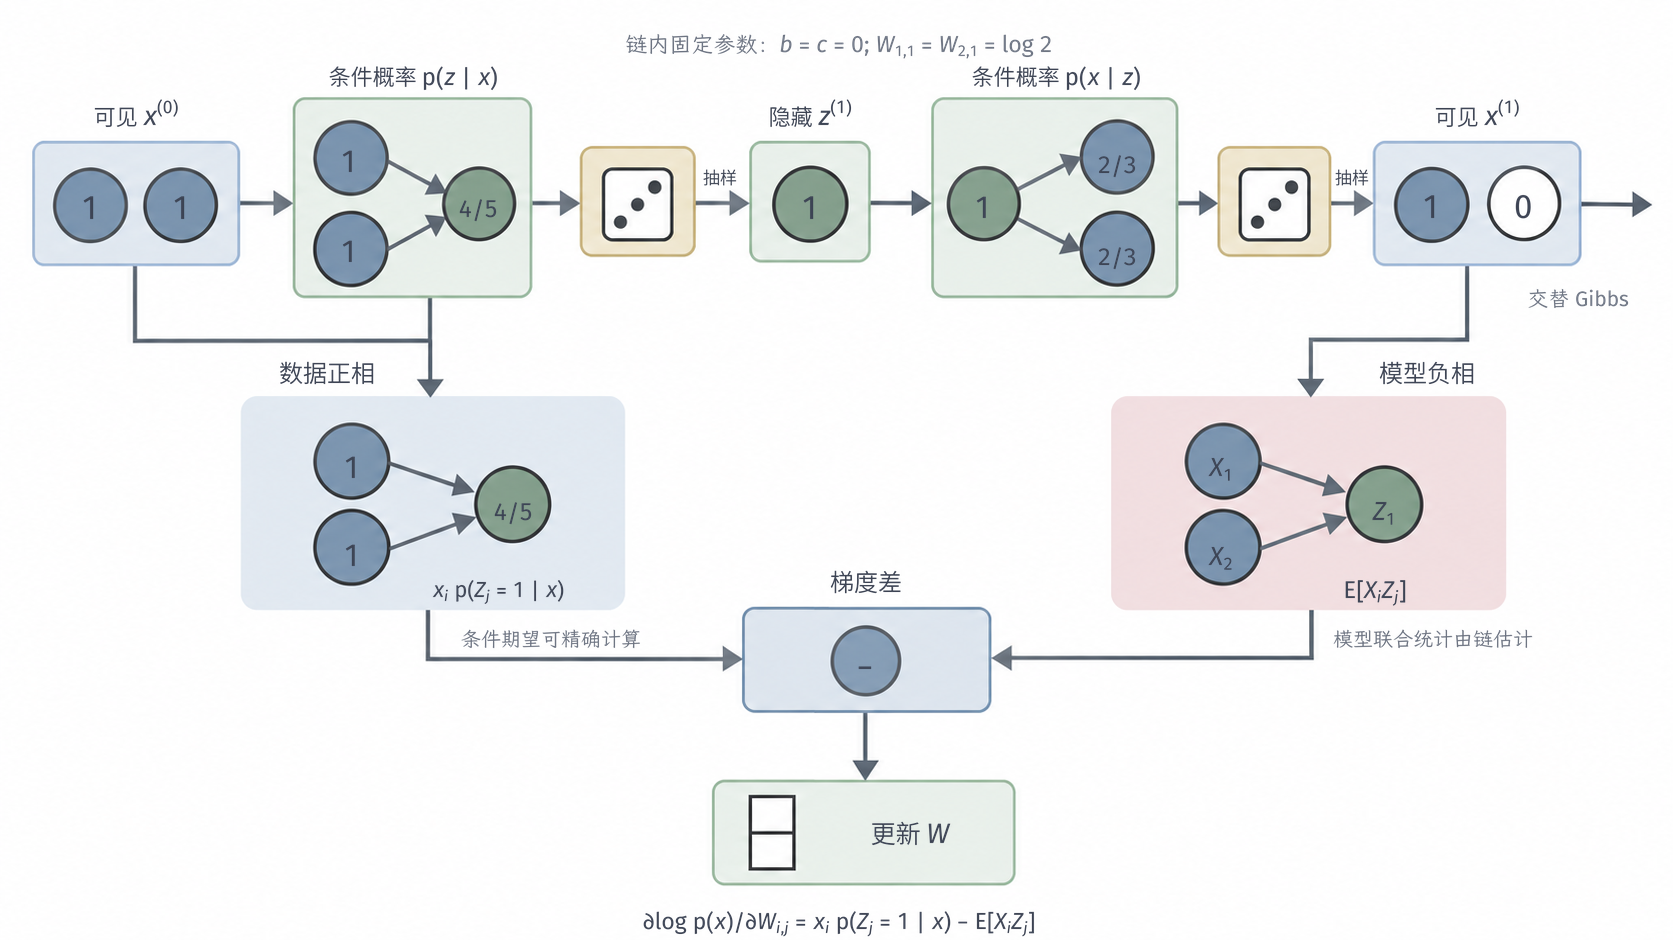
\includegraphics[width=141.647mm]{figures/06-probabilistic-graphical-models/04-models/generated/rbm-alternating-sampling-and-gradient/figure.png}
  \caption{二值RBM中的抽样状态和训练统计。取$b=c=0$、$W_{1,1}=W_{2,1}=\log2$，可见状态$(1,1)$对应隐藏条件概率$4/5$；若抽到$z=1$，可见单元的条件概率各为$2/3$，下一状态可以是$(1,0)$。图中概率与抽样值分别标出。似然梯度以可算的数据统计减去采样估计的模型联合统计，单步重构不能证明混合已完成。}
  \label{fig:rbm-alternating-sampling-and-gradient}
\end{figure*}

\subsection{灵活能量模型}
\label{sec:pgm-energy-models-flexible}

成对二值作用和二次能量限制了相容关系的函数形式。若需要表达更复杂的非线性关系，可以让神经网络为一个配置输出标量能量。\term{神经能量模型}（neural energy-based model）仍按$p_{\bm{\theta}}(\bm{x})\propto e^{-E_{\bm{\theta}}(\bm{x})}$形成分布，改变的是能量函数族。网络的确定性隐藏激活只是计算过程；只有为隐藏量定义了随机分布，才需要把它作为概率潜变量边缘化。

采用$E_{\bm{\theta}}(\bm{x})=\sum_CE_{\bm{\theta},C}(\bm{x}_C)$时，局部网络可以丰富势的形状，同时保留原作用域规定的条件独立性。直接由一个网络读取全部$x_i$而不施加分解，则可能产生全局势；网络内部的计算连线不能代替数据变量的Markov图。函数形式更丰富并不自动降低推断宽度。

连续神经能量能否定义概率，还取决于尾部是否使积分有限。可以在灵活项之外加入二次增长，采用以下充分条件：
\[
  E_{\bm{\theta}}(\bm{x})
    =\frac{\alpha}{2}\lVert\bm{x}\rVert_2^2+r_{\bm{\theta}}(\bm{x}),
  \qquad \alpha>0,\quad r_{\bm{\theta}}(\bm{x})\geq-C,
\]
取有限常数$C$，要求能量可测、在某个正测度集合上有限。上式给出$e^{-E_{\bm{\theta}}(\bm{x})}\leq e^Ce^{-\alpha\lVert\bm{x}\rVert_2^2/2}$，高斯上界保证积分有限，有效支持保证积分为正，合起来得$0<Z_{\bm{\theta}}<\infty$。一般网络不会自动满足这些条件。也可以明确限制到有限体积支持，并保证能量有适当下界。

条件分类得分尚不足以确定输入密度。有限标签上的softmax将$s_k(\bm{x})$转为$p(Y=k\mid\bm{x})$；所有类别得分同时加$c(\bm{x})$，条件概率不变，$\sum_ke^{s_k(\bm{x})}$却改变。因此分类训练不能唯一规定$p(\bm{x})$，单个得分也不能直接解释成$\log p(\bm{x})$。联合能量的支持、归一化对象与训练目标仍需另行给出。

一般神经能量缺少RBM的解析块条件，连续状态可以转用能量对输入的梯度来采样。在无约束$\mathbb{R}^d$上，连续可微能量的一种Langevin离散更新是
\begin{equation}
  \begin{aligned}
    \bm{x}^{(t+1)}
      &=\bm{x}^{(t)}
        -\frac{\varepsilon}{2}
          \nabla_{\bm{x}}E_{\bm{\theta}}(\bm{x}^{(t)})
        +\sqrt{\varepsilon}\,\bm{\xi}^{(t)},\\
    \bm{\xi}^{(t)}&\sim\mathcal{N}(\bm{0},\bm{I}),
       \qquad \varepsilon>0.
  \end{aligned}
  \label{eq:pgm-energy-models-langevin}
\end{equation}
高斯噪声使状态在下降方向之外也能探索邻近区域。固定步长、未经Metropolis校正的离散链一般存在偏差，稳定性还依赖梯度条件；有限步运行另有初始化及混合误差。一次能量梯度求值若耗时$C_E$，一条$k$步负样本链的梯度成本为$O(kC_E)$，远不止一次网络前向求值。Du与Mordatch展示了这类连续神经能量的梯度采样实现，其有限步程序本身不构成任意能量下精确采样的保证\scite{pgm-energy-models-du2019}

对比散度从数据配置启动短链，用终点统计替代模型期望；持久链沿用上轮状态，以跟踪缓慢变化的模型。二者近似了取得模型期望的过程，有限步更新未必等于精确似然梯度。神经能量的形状也会受到这种误差影响：负样本若只覆盖局部区域，其他区域的低能量值可能没有受到训练约束。短链终点随参数变化，忽略其分布导数也是对比散度不一般等于某个固定目标精确梯度的原因（参见第~\ref{chap:pgm-parameter-learning}章）。

若希望避免每轮生成模型链，可以用已知噪声密度$p_{\mathrm{N}}$进行噪声对比估计。其分类对数比为$-E_{\bm{\theta}}(\bm{x})+c-\log[\nu p_{\mathrm{N}}(\bm{x})]$，其中$\nu$是噪声与数据的数量比，$c$作为全局对数归一化参数学习。该目标显式使用噪声密度及采样比例，噪声还须覆盖相关支持，故不等于任意的数据分类训练。高维噪声过易区分时，分类信号可能不足以细化数据附近的密度。

光滑连续密度还可以匹配输入对数密度的梯度。由于$\nabla_{\bm{x}}\log p_{\bm{\theta}}=-\nabla_{\bm{x}}E_{\bm{\theta}}$，分数匹配不需要求$Z$的值。相关导数须可积、分部积分的边界项须为零；满足这些条件时，去掉与参数无关的项后，目标为（推导参见式~\eqref{eq:pgm-parameter-learning-score-matching}）
\[
  \mathbb{E}_{p_*}\!\left[
      \frac12\lVert\nabla_{\bm{x}}E_{\bm{\theta}}(\bm{X})\rVert_2^2
      -\Delta_{\bm{x}}E_{\bm{\theta}}(\bm{X})\right],
\]
这里$p_*$为数据分布，$\Delta_{\bm{x}}$求各坐标二阶偏导之和。省去归一化后，成本转为输入导数，尤其是Hessian迹的计算或估计。标准目标针对连续状态；离散状态或受限支持须另行处理，不能省略相应边界项。训练时无需计算$Z$也不表示训练后已经知道它。加噪数据上的分数学习另见第~\ref{chap:pgm-generative}章。

\subsection{高阶与关系联合模型}
\label{sec:pgm-energy-models-higher-relational}

一组传感器恰有一个激活，或设备、连接及报警共同满足某项规则，都是整组状态的约束。\term{高阶势}（higher-order potential）用至少三个变量共同决定权重。对二值组，记激活数$k_C=\sum_{i\in C}\mathbf{1}\{x_i=+1\}$，可以以$g(k_C)$评价计数。取$\lambda>0$、$k_0\in\{0,\ldots,|C|\}$时，$\lambda\mathbf{1}\{k_C\ne k_0\}$惩罚不符目标计数，$\lambda\mathbf{1}\{0<k_C<|C|\}$惩罚组内不一致。

较大的作用域也可能只是低阶项的另一种写法：$(k_C-k_0)^2$展开后只含常数、一元及成对项。要识别不可约高阶作用，可取三个$\{-1,+1\}$变量，令$p(\bm{x})\propto\exp(\lambda x_1x_2x_3)$、$\lambda\ne0$。乘积符号决定偏好，且满足
\[
  \sum_{\bm{x}\in\{-1,+1\}^3}
     x_1x_2x_3\log p(\bm{x})=8\lambda.
\]
在该求和中，归一化常数对应的项为零，三阶项留下八个$\lambda$。若这个正分布可以仅用原三变量的一元与成对势表示，每项对数势都遗漏至少一个变量，先对遗漏变量求和便得零，左侧因此应为零，与$\lambda\ne0$矛盾。这排除了原变量上的成对改写；增加潜变量后则可能采用另一种表示。

高阶势的内部结构决定局部计算量。任意$r$变量二值稠密因子有$2^r$个表项，对一个变量发送消息通常需遍历另$2^{r-1}$种配置。计数势可以先动态规划汇总其余节点恰有$k$个激活的权重，再乘$e^{-g(k)}$求和，单个输出消息的卷积为$O(r^2)$。这只简化本地因子，未消除其他因子形成的全局环。学习的统计量相应换为计数指示或整体一致性，梯度仍比较经验统计与模型期望。

同一种规则若要用于许多设备，可以将重复因子写成\term{关系模板}（relational template）：规定哪些实体类型及关系参与作用域、哪些实例共享参数。以具体实体替换占位符称为\term{落地}（grounding），得到的还是普通图模型。共享参数减少了参数数量，落地节点和因子仍可能很多，重叠实例也并不独立。

\term{Markov逻辑网络}（Markov logic network, MLN）以逻辑公式组织模板，用成立的落地次数给配置评分。以下限制实体域$D$及谓词集合均有限，并排除产生无限项的函数符号；公式中的自由实体变量遍历域元素。每个落地原子命题是一个Boolean随机变量，配置$\bm{x}$列出全部真值。给模板$r$权重$w_r$、记其落地集合为$\mathcal{I}_r(D)$，联合模型写为
\begin{equation}
  \begin{aligned}
    n_r(\bm{x})
      &=\sum_{g\in\mathcal{I}_r(D)}
           \mathbf{1}\{\text{公式 }r\text{ 在落地 }g\text{ 上为真}\},\\
    E_{\bm{\theta}}(\bm{x})&=-\sum_rw_rn_r(\bm{x}),\\
    p_{\bm{\theta}}(\bm{x})
      &=Z_{\bm{\theta}}^{-1}
          \exp\!\left[\sum_rw_rn_r(\bm{x})\right].
  \end{aligned}
  \label{eq:pgm-energy-models-mln}
\end{equation}
逻辑蕴含说明公式何时成立，不是有向概率边。正权重奖励满足公式的配置；权重有限时，违反公式的实例仍可有非零概率，并非硬性规则。

模板$\operatorname{Fault}(a)\Rightarrow\operatorname{Alarm}(a)$涉及同一设备的故障与报警。若要表达跨设备的相互作用，还可以使用
\[
  \operatorname{Linked}(a,b)\land\operatorname{Fault}(a)
       \ \Rightarrow\ \operatorname{Fault}(b)
\]
将$(a,b)=(u,v)$代入后，连接及两个故障原子共同进入一个因子；连接未观测时，它构成三阶作用。概率图连线说明命题共同参与某个因子，不能直接解释成实体存在物理连接。将连接设为证据会简化因子，所做的是原联合分布的条件化。

逻辑权重与规则概率也需区分。只给一个设备使用首个模板，取$w=\log4$且无其他势，以$F,A$记故障、报警真值。配置$(0,0),(0,1),(1,0),(1,1)$中，三个满足蕴含的权重为$4$，违反配置$(1,0)$的权重为$1$，所以$Z=13$。公式成立概率为$12/13$，条件报警概率$p(A=1\mid F=1)=4/5$，边缘报警概率$p(A=1)=8/13$。三项查询各有条件，不能把权重直接当作其中任何一个概率；重叠模板还会使查询依赖周围证据。

学习$w_r$时，似然梯度累加全部落地实例，比较观测的$n_r$与模型期望。完整观测可以使用伪似然；部分命题未观测时，数据统计也需后验推断。消元、近似消息及采样作用于落地后的模型。域大小$N=|D|$、模板有$q$个实体占位符时，实例数可能达$O(N^q)$，精确推断还受落地图宽度约束。模板简短和参数共享并未消除这些成本，MLN的构造及伪似然学习参见原始工作\scite{pgm-energy-models-richardson2006}

硬规则排除违反配置；相互矛盾时可能没有正权配置，即$Z=0$，可行区域分离时单点采样也可能无法穿越。软规则虽避免这种排除，扩大实体域仍会改变落地次数与模板的相对作用，复用原权重未必保持原边缘概率。关系共享规定重复结构及参数合并，不自动保证不同域规模下的概率一致性。

\section{条件能量模型}
\label{sec:pgm-energy-models-conditional-models}

若温度、历史摘要和传感器类型已经给定，检测任务可以只预测异常标签。为这些输入另拟联合分布未必是必要步骤。条件能量将输入作为已知量，专门表达标签之间的相容性；标签配置共同竞争概率质量，仍须处理全局输出归一化。

\subsection{条件随机场的定义}
\label{sec:pgm-energy-models-crf-definition}

固定输入之后，可以用无向图规定标签的条件独立关系。满足这种Markov性质的条件分布称为\term{条件随机场}（conditional random field, CRF），通常通过输入相关的团势构造：
\begin{equation}
  \begin{aligned}
    p_{\bm{\theta}}(\bm{y}\mid\bm{x})
      &=\frac{1}{Z_{\bm{\theta}}(\bm{x})}
          \prod_{C\in\mathcal{C}}
             \psi_{\bm{\theta},C}(\bm{y}_C,\bm{x}),\\
    E_{\bm{\theta}}(\bm{y},\bm{x})
      &=-\sum_{C\in\mathcal{C}}
             \log\psi_{\bm{\theta},C}(\bm{y}_C,\bm{x}).
  \end{aligned}
  \label{eq:pgm-energy-models-crf-factors}
\end{equation}
该图只以输出变量为节点。固定输入，若$S$分离$A$、$B$，则$\bm{Y}_A\perp\bm{Y}_B\mid(\bm{Y}_S,\bm{x})$。完整输入可以被多个势或序列编码器读取；标签作用域由一个势同时涉及哪些未知标签决定，不能从输入编码器的连线推定。

既有联合Markov模型$p(\bm{x},\bm{y})$条件化后也能给出CRF形式，直接条件拟合则只学习$p(\bm{y}\mid\bm{x})$，不同时约束$p(\bm{x})$。反向组成联合分布时，必须为CRF另选输入分布。输入缺失需要边缘化时，同样缺少其分布，单凭条件标签模型无法完成这项查询。

常用的线性形式为$\log\psi_{\bm{\theta},C}=\bm{\theta}^\top\bm{f}_C(\bm{x},\bm{y}_C)$，各作用域可以共享参数。给定完整标签记录$\{(\bm{x}_r,\bm{y}_r)\}_{r=1}^n$，比较观测特征得分与该输入下全部标签的权重总量，条件对数似然为
\begin{equation}
  \ell_{\mathrm{cond}}(\bm{\theta})
    =\sum_{r=1}^n
       \left[
        \sum_C\bm{\theta}^\top
                    \bm{f}_C(\bm{x}_r,\bm{y}_{r,C})
        -\log Z_{\bm{\theta}}(\bm{x}_r)
       \right].
  \label{eq:pgm-energy-models-crf-likelihood}
\end{equation}
不同输入一般给出不同配分函数，梯度要逐条计算条件标签边缘及期望特征，推断因而反复参与训练。固定特征、完整标签的线性参数化使对数似然为凹函数，有限最优解仍取决于可分离性与正则化；可训练神经特征或未观测标签的边缘化则不保留一般凹性结论（梯度推导参见第~\ref{sec:pgm-parameter-learning-conditional}节）。CRF的完整表述见Sutton与McCallum\scite{pgm-energy-models-sutton2012}

\subsection{线性链条件随机场}
\label{sec:pgm-energy-models-linear-chain}

顺序标签只保留相邻相互作用时，输出图是一条链。\term{线性链条件随机场}（linear-chain CRF）将得分分为单点状态项与相邻转移项；序列长度为$T$、$y_t\in\{1,\ldots,K\}$时，写成
\begin{equation}
  \begin{aligned}
    f_{\bm{\theta}}(\bm{y},\bm{x})
      &=\sum_{t=1}^T a_t(y_t;\bm{x})
        +\sum_{t=2}^T b_t(y_{t-1},y_t;\bm{x}),\\
    p_{\bm{\theta}}(\bm{y}\mid\bm{x})
      &\propto e^{f_{\bm{\theta}}(\bm{y},\bm{x})}.
  \end{aligned}
  \label{eq:pgm-energy-models-chain-score}
\end{equation}
$a_t$评价输入与当前标签，$b_t$评价相邻标签组合。记$\phi_t(k)=e^{a_t(k;\bm{x})}$、$\psi_t(j,k)=e^{b_t(j,k;\bm{x})}$，暂略参数下标；首尾偏好可分别计入$a_1$、$a_T$。“转移”在这里是标签相容势，无须满足$\sum_k\psi_t(j,k)=1$，也不规定标签的因果生成顺序。

要汇总所有标签序列，可将具有相同末标签的前缀合并。\term{前向消息}（forward message）$\alpha_t(k)$保存以$y_t=k$结束的长度$t$前缀权重总和。按前一标签分组，再加上当前状态势和边势，得到
\begin{equation}
  \begin{aligned}
    \alpha_1(k)&=\phi_1(k),\\
    \alpha_t(k)&=\phi_t(k)
       \sum_{j=1}^K\alpha_{t-1}(j)\psi_t(j,k),
       \qquad t=2,\ldots,T,\\
    Z_{\bm{\theta}}(\bm{x})&=\sum_{k=1}^K\alpha_T(k).
  \end{aligned}
  \label{eq:pgm-energy-models-forward}
\end{equation}
每个长度$t$前缀只对应一个末标签对$(j,k)$，新增权重是旧前缀权重乘状态势及边势。分组没有遗漏或重复，结合初始消息即可归纳证明$\alpha_t$确为全部相应前缀权重之和。

单点边缘还需要当前位置右侧的证据。以$\beta_t(j)$保存固定$y_t=j$时、$t+1$至$T$的后缀权重和，排除当前位置的状态势，则
\begin{equation}
  \begin{aligned}
    \beta_T(j)&=1,\\
    \beta_t(j)&=\sum_{k=1}^K
         \psi_{t+1}(j,k)\phi_{t+1}(k)\beta_{t+1}(k),\\
    p(Y_t=k\mid\bm{x})
      &=\frac{\alpha_t(k)\beta_t(k)}{Z_{\bm{\theta}}(\bm{x})}.
  \end{aligned}
  \label{eq:pgm-energy-models-backward}
\end{equation}
相邻标签固定后，左右部分分别由前向和后向消息汇总，将边势和右端状态势接入可得
\begin{equation}
  p(Y_{t-1}=j,Y_t=k\mid\bm{x})
   =\frac{\alpha_{t-1}(j)\psi_t(j,k)
                   \phi_t(k)\beta_t(k)}
          {Z_{\bm{\theta}}(\bm{x})}.
  \label{eq:pgm-energy-models-edge-marginal}
\end{equation}
状态边缘与边边缘恰好足以计算式~\eqref{eq:pgm-energy-models-chain-score}中局部特征的模型期望；求和消元的通用原理见第~\ref{chap:pgm-elimination}章。

现在沿用三位置例子，把未知状态改记为标签$y_t\in\{-1,+1\}$。边势仍在同号时为$3$、异号时为$1$；某个固定输入给出的状态势，按$(-1,+1)$排列，三个位置分别取$(1,2)$、$(1,1)$、$(1,3)$。输入偏好首尾为正，中间位置没有局部偏好。表~\ref{tab:pgm-energy-models-chain-weights}列出全部配置，使归一化和解码都可直接核验。

\begin{table}[htbp]
  \centering
  \begin{tabular}{crr}
    \toprule
    状态或标签配置 & 联合权重$w_0$ & 条件权重$w_{\bm{x}}$\\
    \midrule
    $(-,-,-)$ & $9$ & $9$\\
    $(-,-,+)$ & $3$ & $9$\\
    $(-,+,-)$ & $1$ & $1$\\
    $(-,+,+)$ & $3$ & $9$\\
    $(+,-,-)$ & $3$ & $6$\\
    $(+,-,+)$ & $1$ & $6$\\
    $(+,+,-)$ & $3$ & $6$\\
    $(+,+,+)$ & $9$ & $54$\\
    \midrule
    总和 & $32$ & $100$\\
    \bottomrule
  \end{tabular}
  \caption{同一组相邻势下的联合与条件权重。符号$+$、$-$分别表示$+1$、$-1$；条件列在联合列上乘以固定输入给出的三项状态势。两列须分别除以各自总和，不能把状态势误当作已归一化的标签概率。}
  \label{tab:pgm-energy-models-chain-weights}
\end{table}

把两个标签对应的消息值按$(-1,+1)$组成向量，前向递推给出$\bm{\alpha}_1=(1,2)$、$\bm{\alpha}_2=(5,7)$、$\bm{\alpha}_3=(22,78)$，例如$\alpha_2(+1)=1(1\times1+2\times3)=7$。因此$Z(\bm{x})=100$。后向递推给出$\bm{\beta}_3=(1,1)$、$\bm{\beta}_2=(6,10)$、$\bm{\beta}_1=(28,36)$，所以
\[
  p(Y_2=+1\mid\bm{x})=\frac{7\times10}{100}=0.7.
\]
中间位置没有自己的类别偏好，却从两侧输入获得了正类证据。两条边同号的边缘概率都为$0.78$；若训练标签是$(+,+,+)$，共享的同号得分参数$\eta=\log3$在该记录上的似然梯度就是$2-2\times0.78=0.44$，推动模型增加同号序列的相对权重。这里仅实例化期望特征，并未将不同边视为独立训练记录。

如果任务是找最可能的完整标签序列，则应把前向求和换成取最大，并保存前驱。这是\term{Viterbi算法}（Viterbi algorithm），即在链上复用最优前缀的动态规划。用对数得分避免连乘，有
\begin{equation}
  \begin{aligned}
    \delta_1(k)&=a_1(k;\bm{x}),\\
    \delta_t(k)&=a_t(k;\bm{x})
       +\max_j\{\delta_{t-1}(j)+b_t(j,k;\bm{x})\}.
  \end{aligned}
  \label{eq:pgm-energy-models-viterbi}
\end{equation}
对每个$(t,k)$保存达到最大值的$j$，从$\argmax_k\delta_T(k)$向前回溯；平局可按固定标签顺序选择一个最优解。在数值例子中，将$\exp[\delta_t(k)]$按标签$(-1,+1)$排列，三步依次为$(1,2),(3,6),(9,54)$，回溯得到$(+,+,+)$，概率为$0.54$。逐位置选择边缘最大的标签优化的是逐位置错误的期望，不是完整序列概率；本例二者恰好相同，不能据此将两种解码等同。最大积也只适用于这里对全部未知标签的联合最大化；若另有潜变量要先求和，需重新区分联合最优与边缘MAP。

前向、后向和Viterbi各需要$O(TK^2)$时间。仅求配分函数时消息空间为$O(K)$，保留全部节点边缘或解码回溯通常需要$O(TK)$消息或前驱空间；若存储所有稠密边势，另需$O(TK^2)$空间。长序列应使用对数域的log-sum-exp，或逐步缩放并记录缩放常数，否则数值下溢会破坏归一化。每条训练记录的梯度也需要同量级的前向后向推断，特征提取或神经编码器的成本另计。

输入的远程信息可以进入$a_t$，而不改变上述标签递推；直接加入$y_t$与远处未知标签的耦合则会改变图结构。线性链适合局部标签依赖，但不能独立表达任意长程标签约束。与局部归一化的逐状态分类器相比，CRF让整个输出序列共同竞争概率质量；代价是每次训练与概率查询都要处理完整链的归一化，而不是分别拟合各个状态的分类概率\scite{pgm-energy-models-sutton2012}

\subsection{半Markov与高阶条件随机场}
\label{sec:pgm-energy-models-semi-higher}

有些输出对象本来就是片段：一个异常区间的长度、区间内部温度的整体形状，都难以只用相邻标签对评价。\term{半Markov条件随机场}（semi-Markov CRF）将基本输出单位改为带标签的连续片段，让一个势同时评价片段的起止位置、整体输入及相邻片段标签。它仍对全部合法分段作一次条件归一化，不是先确定边界再各自分类。

设一次分段为$\bm{s}=((a_\ell,b_\ell,k_\ell))_{\ell=1}^M$，片段无重叠、无空隙地覆盖$1,\ldots,T$，即$a_1=1$、$a_{\ell+1}=b_\ell+1$、$b_M=T$，长度满足$1\leq b_\ell-a_\ell+1\leq L$。$k_\ell\in\{1,\ldots,K\}$是片段标签，$M$随分段变化；用$k_0=0$表示起始哨兵标签。令$g(a,b,j,k;\bm{x})$为前一片段标签$j$接上当前$[a,b]$、标签$k$的得分，则
\begin{equation}
  p_{\bm{\theta}}(\bm{s}\mid\bm{x})
   =\frac{\exp\!\left[
        \sum_{\ell=1}^M
          g(a_\ell,b_\ell,k_{\ell-1},k_\ell;\bm{x})
                    \right]}
          {Z_{\bm{\theta}}(\bm{x})}.
  \label{eq:pgm-energy-models-semi-distribution}
\end{equation}
配分函数对所有合法$\bm{s}$求和，包括不同边界和不同片段数。这里允许相邻片段有相同标签；若任务规定同标签相邻片段必须合并，就应把这项约束写入合法分段集合，算法也要禁止相应转移。

动态规划在片段边界处汇总信息。令$A_t(k)$为覆盖前$t$个位置且末片段标签为$k$的权重和，设$A_0(0)=1$、$A_0(k)=0$（$k>0$），并令$t>0$时$A_t(0)=0$。则
\begin{equation}
  A_t(k)=
    \sum_{\ell=1}^{\min(L,t)}\sum_{j=0}^K
       A_{t-\ell}(j)
       e^{g(t-\ell+1,t,j,k;\bm{x})}.
  \label{eq:pgm-energy-models-semi-forward}
\end{equation}
仅在首片段允许$j=0$。递推枚举末片段长度$\ell$和前一片段标签$j$，每个完整前缀都有唯一的这种拆分，因此没有重复计数；最终$Z(\bm{x})=\sum_{k=1}^KA_T(k)$。将求和改成最大并记录长度和标签，就能回溯最优分段。

学习片段特征还需要片段边缘。记$B_b(k)$为边界$b$之后、前一片段标签固定为$k$的所有后缀权重和，取$B_T(k)=1$，按下一片段的长度与标签反向递推即可。一次相邻片段连接的边缘概率为
\[
  \frac{A_{a-1}(j)
           e^{g(a,b,j,k;\bm{x})}B_b(k)}
       {Z_{\bm{\theta}}(\bm{x})}.
\]
这使长度、片段形状及片段转移等特征的期望可计算。若边界与片段标签全部已知，训练使用式~\eqref{eq:pgm-energy-models-semi-distribution}的对数概率；若只给定较粗标签、边界仍未知，分子也须对相容分段求和，不能拿一个最优分段代替这项边缘化。

一个极小例子可以核查“分段”与“逐点标签”的区别。取$T=3,K=1,L=2$，长度$1$片段的权重为$1$，长度$2$片段的权重为$2$，无其他得分。合法长度序列为$(1,1,1),(1,2),(2,1)$，权重分别为$1,2,2$。递推得到$A_1=1,A_2=3,A_3=5$，所以配分函数为$5$，位置$1$后出现边界的概率为$(1+2)/5=3/5$。所有分段都给出同一组逐点标签，但边界的不确定性仍然存在；长度上限排除的是一个长度$3$的单片段，不是三个同标签位置组成的序列。

若每个候选片段得分已可常数时间读取，一次前向或后向计算为$O(TLK^2)$，保存全部边界消息需要$O(TK)$空间；预先存储所有含转移的片段得分则可达$O(TLK^2)$。只求配分函数时可以滚动保留最近$L$个边界。若计算片段特征本身需要扫描片段内部，必须额外计入该成本。长度上限降低计算量，也会排除模型本来可能需要的长片段；不能仅因动态规划精确，就忽略候选集合的限制\scite{pgm-energy-models-sarawagi2004}

另一种扩展不改变逐点输出，而是扩大未知标签的作用域。\term{高阶条件随机场}（higher-order CRF）可以用$(r+1)$个连续标签共同决定一个势，即$E=-\sum_t f_t(y_{t-r},\ldots,y_t;\bm{x})$，序列起点使用固定哨兵补齐。在这种有限记忆结构下，消息需保留最近$r$个标签；每个位置有$K^r$种历史，每种历史接上$K$种新标签，所以朴素精确递推为$O(TK^{r+1})$时间、$O(K^r)$滚动消息空间。扩展状态间只能按共享后缀相接，不必建立任意$K^r\times K^r$稠密转移表。

图~\ref{fig:pgm-energy-models-crf-scopes}比较了这两种扩展。片段模型通过增加可选长度来表达持续区间；高阶链通过增加消息保留的标签组合来表达更长依赖。二者还可以组合，神经网络也可以参数化其中的局部得分，但其成本不能只用“一阶链”或“神经网络”的名称判断。若高阶势跨越任意远的未知标签，有限记忆递推也未必仍然适用。

\begin{figure}[htbp]
  \centering
  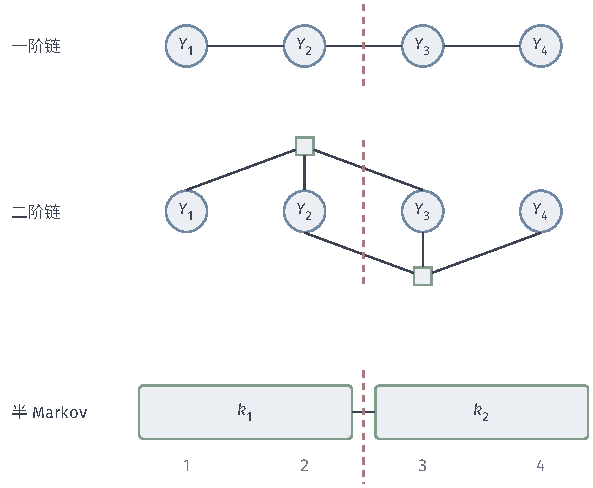
\includegraphics[width=100.404mm]{figures/06-probabilistic-graphical-models/04-models/tikz/pgm-energy-models-crf-scopes/figure.pdf}
  \caption{输出作用域的三种选择。一阶链的切分处只需保留一个标签；二阶链中，跨切分处的三元势需要保留两个标签。半Markov模型按片段边界递推，图中展示一种$[1,2]$与$[3,4]$的分段，推断时还须对其他合法边界求和。}
  \label{fig:pgm-energy-models-crf-scopes}
\end{figure}

\subsection{一般图与关系条件随机场}
\label{sec:pgm-energy-models-general-relational}

当输出对应二维检测网格，或分别属于存在连接关系的设备时，一条链无法保留所有必要相互作用。一般图CRF仍按式~\eqref{eq:pgm-energy-models-crf-factors}分解，但图由输出之间的关系决定。关系CRF进一步将这些作用域写成模板：已知设备属性、连接关系和图结构都进入输入，未知量则是待预测的标签。

例如，给每个设备一个标签$Y_i$，让设备属性产生一元势，让每条已知连接复用同一个相邻标签势。更一般地，若输入$\bm{x}$决定模板$r$的实例集合$\mathcal{I}_r(\bm{x})$，可写
\begin{equation}
  E_{\bm{\theta}}(\bm{y},\bm{x})
   =-\sum_r\sum_{g\in\mathcal{I}_r(\bm{x})}
        \bm{\theta}_r^\top
             \bm{f}_r(\bm{x}_g,\bm{y}_g).
  \label{eq:pgm-energy-models-relational-crf}
\end{equation}
这里$g$标识一组具体实体及关系所选出的作用域，$\bm{x}_g$是相关已知特征，$\bm{y}_g$是参与该因子的未知标签。同一个$\bm{\theta}_r$从全部实例汇总学习信号；不同实例可以重叠，不因此成为独立样本。Taskar等人的关系Markov网络工作给出了这类条件建模与集体分类的代表形式\scite{pgm-energy-models-taskar2002}

固定关系输入并没有自动使输出图无环。例如设备之间的连接形成一个闭环，标签势也会形成闭环。精确推断可以用第~\ref{chap:pgm-junction-tree}章的团树方法，复杂度由消元后的最大作用域决定。若每个标签有$K$种取值、所选消元序的诱导宽度为$w$，主要运算一般含$K^{w+1}$；简单环仍有较小宽度，并非出现一个环就必须近似。密集跨设备约束或大型高阶势则可能使团树不再可承受。

计算受限时，可以用第~\ref{chap:pgm-variational}章的平均场、环置信传播或最大化松弛，也可以用第~\ref{chap:pgm-sampling}章的采样。需要标签概率或条件似然梯度时，目标是边缘和期望；只需要完整标签的最优配置时，目标是最大化得分。对后者有效的图割或整数优化程序，不一定能返回前者。一般图上的环消息可能不收敛，即使收敛也不一般等于精确边缘；用其结果训练时，应明确正在使用近似梯度或近似配分函数。

关系模型还会放大建模假设的影响。若所有连接都被解释为“标签应相同”，实际连接却经常跨越不同故障类型，集体推断会把偏差传播到多个节点。度较大的节点参与更多势，局部错误也可能被多次计入；这需要在特征和参数共享方式上处理，不能靠扩大消息迭代次数修正。已知连接只是输入时，模型也没有定义未知连接的生成概率，不能直接把标签推断扩展成连接生成。

训练与评价应以任务中的完整关系结构为单位说明数据来源。在同一张大图上划分已标注与未标注节点可以构成合法的传导预测任务，但它不同于预测全新独立图；测试标签不得通过邻域特征进入训练。若只观测部分训练标签，需在条件似然分子中对其他标签求和，又会带来后验推断和通常非凹的优化。关系共享有助于合并重复模式的信息，不消除相关性、推断误差或划分泄漏。

\section{模型比较}
\label{sec:pgm-energy-models-comparison}

这些模型都把局部得分组合成全局概率，差别应落实到哪些变量参与归一化、哪些变量被观测，以及积分或求和能否利用结构。表~\ref{tab:pgm-energy-models-comparison}列出本章所讨论的代表设定；同一实例可以同时具有多行中的属性，例如神经高阶关系CRF仍然属于条件能量模型，不能把表中名称当作互斥分类。

\begin{table*}[htbp]
  \centering
  \small
  \begin{tabularx}{\linewidth}{p{27mm}p{19mm}p{24mm}p{24mm}X}
    \toprule
    代表设定 & 归一化对象 & 变量与潜变量 & 势的作用域 & 可计算性与主要限制\\
    \midrule
    Ising／Potts & 全部状态 & 离散；此处全观测 & 一元、成对 & 树上精确；一般图的全局求和与强耦合采样可能昂贵\\
    高斯MRF & 全部状态 & 连续；此处全观测 & 二次能量 & 正定精度下可解析归一化；矩阵填充与单峰限制\\
    BM／RBM & 可见与隐藏状态 & 二值；含潜变量 & 联合空间成对 & RBM的块条件与自由能可算，联合配分函数一般仍难\\
    神经联合能量 & 全部状态 & 可离散或连续；潜变量可选 & 局部或全局 & 网络求值不等于归一化；尾部、采样和学习偏差均需控制\\
    MLN & 落地命题配置 & Boolean；可有未观测命题 & 模板决定阶数 & 参数共享不消除落地数量及推断宽度的增长\\
    线性链CRF & 给定输入的标签 & 离散；此处完整标签 & 一元、相邻成对 & $O(TK^2)$精确归一化；不直接表示任意远程标签约束\\
    半Markov／高阶链CRF & 分段或标签组合 & 离散；边界可未观测 & 片段或连续高阶 & 分别受$L$与$K^r$影响；有限结构下可精确递推\\
    一般图关系CRF & 给定关系输入的标签 & 此处离散；标签可缺失 & 成对或高阶 & 低宽度可精确；宽图依赖近似推断且须重复用于学习\\
    \bottomrule
  \end{tabularx}
  \caption{按本章具体设定比较模型。$T$为序列长度，$K$为标签数，$L$为最大片段长度，$r$为高阶链保留的历史标签数。潜变量、势阶数与参数化方式可以组合；条件无向模型也可以有连续输出，此表不穷尽这些组合。}
  \label{tab:pgm-energy-models-comparison}
\end{table*}

联合与条件的选择主要由查询决定。若需要解释整组测量、补全不同类型的未知变量或生成新的联合配置，就需要相应联合模型；若始终固定输入，只评价标签预测，直接条件建模避免额外约束输入分布。条件化不等于局部归一化，也不保证计算更便宜：一个复杂的输出图仍可能难以求和，而且训练中每个不同输入都有自己的$Z_{\bm{\theta}}(\bm{x})$。

表示能力与计算代价也不能只靠“势是否成对”判断。GMRF即使有环也能借助二次结构计算，RBM即使只有成对边也可能难以归一化；计数高阶势可以利用卷积，任意高阶表却要付出指数存储。神经网络扩大局部函数族时可以保持原图，直接给全局配置打分则可能失去稀疏分解。真正相关的是运算的代数形式、未知变量作用域和消元后的宽度。

学习的主要障碍与这些推断结构对应。完整离散联合模型需要模型期望；BM还需要数据条件下的隐藏后验，RBM只简化了后者；连续神经能量常把计算预算花在生成负样本或求输入导数上。链式CRF虽可精确求期望，长序列、大标签集和大量样本仍使反复推断昂贵。判断一套训练流程时，应分别检查能量是否定义了合法分布、所需查询能否求出，以及近似训练究竟偏离了什么目标；这些问题不能用一个训练损失数值代替。

\section{本章小结}
\label{sec:pgm-energy-models-summary}

局部相容信息之所以能成为整组状态的概率，是因为所有配置的权重共同参与归一化。能量只是这些权重的负对数表示；绝对能量零点可以改变，状态之间的能量差以及归一化后的概率才决定模型行为。三位置例子中，未加输入时的配分函数为$32$；固定新的输入相关状态势后，标签配分函数变成$100$，中间位置即使没有自己的偏好，也会通过相邻作用获得两侧证据。

联合无向模型与条件无向模型区分的是求和对象，不是势是否复杂。引入潜变量可以把简单联合相互作用转成复杂边缘依赖，RBM的二部结构使隐藏后验和自由能可算，却未消除联合归一化。高阶势与关系模板可以表达整体约束，但须检查作用域、落地规模与硬约束的可行性。神经能量允许更灵活的函数形状，也需要单独保证可归一化并控制采样或替代学习准则的误差。

条件能量模型把输入视为给定，并不削弱对输出依赖的建模。链、片段和有限阶历史之所以可精确计算，是因为递推只需保留有限边界信息；一般输出图则仍受推断宽度限制。由此回到开篇的问题：是否需要解释测量的生成分布，决定选用联合无向模型还是条件无向模型；需要保留何种相互作用，以及能承受哪种求和或采样代价，决定其内部结构。模型选择、推断与参数学习必须在这两个层次上相互配合。

同样是序列结构，也可以先描述潜状态怎样演化，再描述观测怎样产生。第~\ref{chap:pgm-dynamic}章采用这一有向生成方式，继续使用链上的求和与最大化，但其局部因子是转移、发射分布，而非给定完整输入后的任意标签势。这一区别决定了模型能否直接预测未来观测。

\paragraph{扩展阅读}
Bishop的PRML及Murphy的教材补充能量模型、配分函数和采样训练。阅读时应把评价未归一化分数、计算概率以及估计梯度所需的模型期望分开，不能用前者的容易计算推断后二者\scite{bishop2006,pgm-murphy2012}
